% The "%" character denotes a comment
% This file was written by Nathan Moore, Winona State University
% as a template for how lab reports might be written in LaTeX.
% style choices originally come from the American Journal of Physics's
% sample submission file, http://ajp.dickinson.edu/Contributors/manFormat.html
%
%
\documentclass[prb,preprint]{revtex4-1}
\usepackage{amsmath}  % needed for \tfrac, \bmatrix, etc.
\usepackage{amsfonts} % needed for bold Greek, Fraktur, and blackboard bold
\usepackage{graphicx} % needed for figures

%these are some macros (shortcuts)
\newcommand{\bea}{\begin{eqnarray}}
\newcommand{\eea}{\end{eqnarray}}
\newcommand{\be}{\begin{equation}}
\newcommand{\ee}{\end{equation}}

\begin{document}

\title{Electronics Lab 08: Load Lines}
\author{Adam Stammer}
%\email{adam.stammer@go.winona.edu}

\date{\today}

%if you include an abstract, it goes here
%\begin{abstract}
%\end{abstract}

\maketitle


%These are my general reccomendations for an undergraduate lab report in Physics. 
%
%\textbf{Purpose}
%The lab report should start with a purpose statement.  Briefly 
%provide the necessary background and explain what problem your are trying to 
%solve/investigate.
%
%\textbf{Conclusions} Don't be coy, cut to the point right away and state what you found. This should be breif.
%
%\textbf{Theory} We never just measure stuff in Physics.  There's always a 
%theoretical idea behind the measurement we're making.  Explain  the ideas 
%behind your work, starting at the level of a successful Physics 221/222 
%student.
%
%\textbf{Data} Sketch out, in words and pictures, the apparatus you used to take data.  Report the data, graphically, if possible, and state the uncertainties  in your measurement.  Don't provide pages of computer printout here. Data tables shouldn't be your first choice when it comes to communicating your measurements.\cite{Tufte}
%
%\textbf{Analysis} With data presented, describe how the theory agrees/disagrees with 
%the data you took.  Normally this is accomplished with a fit line (or math 
%model) that is interpreted.
%
%\textbf{Limitations and Recommendations} Every measurement has limitations and it is only honest to report them to the reader.  ``Human Error'' is a meaningless statement.  After your analysis is complete, revisit the purpose statement.  This is the place to more forcefully argue your conclusions.    
%
%Notes: 
%Writing in the first person, eg ``I" or ``We," is fine.
%
%\newpage
%\textbf{Example Lab Report:}

\section{Theory}

We connected a 5 Volt power source across the base and emitter of a 2222 transistor in series with a resistor. The resistor served to limit and control the current through the transistor as we analyzed it. Varying the resistor was our means to vary the current going into the base and out of the emitter. Since this is simply a PN junction, Shockley's equation, $i_{d} \approx I_{s}e^{\frac{V_{D}}{V_{T}}}$, to help analyze our data. 

Now if we solve Shockley's Equation for $V_{D}$ we get the following.
\begin{equation}
V_{D}=\ln{(\frac{i_{D}}{I_{s}})nV_{T}}
\end{equation}
\begin{equation}
V_{D}=nV_{T}(\ln{i_{D}}-\ln{Is})
\end{equation}

Taking this a step further to get it into a linear $y=mx+b$ form we see the following.

\begin{equation}
\ln{i_{D}}=\frac{1}{nV_{T}}V_{D}+\ln{I_{s}}
\end{equation}

This clearly shows us a linear relationship with a slope of $\frac{1}{nVt}$, and a y intercept of $\ln{I_{s}}$. We can compare this without collected data once it is properly fit a linear trend.

\section{Data}

The collected data was then graphed with error bars as seen below. Layering the $i_{D}$ in a natural log allows our $V_{D} vs i_{D}$ graph to actually have a linear relationship.

\begin{figure}[ht]
\centering
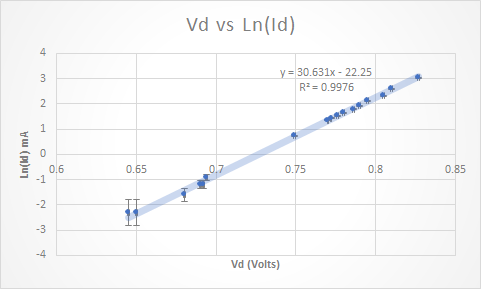
\includegraphics[width=6in]{vdlnid.png}
\caption{Collected Data Graphed in Excel}
\label{fig1}
\end{figure}

A trendline, $y=30.631x-22.25$, was then made to fit the data from which we can extrapolate some valuable data, notably the y intercept and the slope.

If we take our extrapolated y intercept of -22.25 and set it equal to our theoretical intercept of $\ln{I_{s}}$ we can solve for the saturation current, ($I_{s}$), of our transistor.

\begin{equation}
\ln{I_{s}} = -22.25
\end{equation}
\begin{equation}
I_{s} = e^{-22.25} = 2.1724*10^{-10} mA
\end{equation}

A saturation current of $2.1724*10^{-13}$ milliAmps is within our range of reasonable numbers.

We can also use our slope of 30.631 to solve for $V_{T}$ if we assume our value of n. In this case let's assume $n=1$.

\begin{equation}
\frac{1}{nV_{T}} = 30.631
\end{equation}
\begin{equation}
V_{T} = 0.032647
\end{equation}

While 32.647 milliVolts isn't outside of our range of possibilities, it seems a tad high to me. 26mV is already a higher estimation for $V_{T}$ at room temperature. We could instead measure the temperature to directly find $V_{T}$ which could then be used to find n itself. If we do this we find n to be $\approx1.2821$ when we assume a $V_{T}$ of 26mV.

Since we were able to solve for the saturation current, assuming we know $V_{T}$ we could alternatively use Shockley's equation to solve for n.

%\begin{thebibliography}{99}
% The numeral (here 99) in curly braces is nominally the number of entries in
% the bibliography. It's supposed to affect the amount of space around the
% numerical labels, so only the number of digits should matter--and even that
% seems to make no discernible difference.
%Not Requested
%\end{thebibliography}

\end{document}
